%%%%%%%%%%%%%%%%%%%%%%%%%%%%%%%%%%%%%%%%%%%%%%%%%%%%%%%%%%%%%%%%%%%%%%%
%%%%  Load the document class and packages                         %%%%
%%%%%%%%%%%%%%%%%%%%%%%%%%%%%%%%%%%%%%%%%%%%%%%%%%%%%%%%%%%%%%%%%%%%%%%
\documentclass[a4paper]{report}
\usepackage{epsfig}            % to insert PostScript figures
\graphicspath{ 
	{./figures/} 
}

%Change figure names
\renewcommand{\figurename}{Fig}

\usepackage[bf,footnotesize]{caption} % make captions small and label bold

\addtocounter{chapter}{1} %Because starting at zero is silly
\makeatletter
\renewcommand{\thesection}{\@arabic\c@section}
\renewcommand{\thefigure}{\@arabic\c@figure}
\makeatother

\usepackage{titlesec} %change spacing before and after sections
%format: \titlespacing*{<command>}{<left>}{<before-sep>}{<after-sep>}
\titlespacing*{\section}{0pt}{11mm plus 1ex minus .2ex}{6mm plus .2ex}
\titlespacing*{\subsection}{0pt}{9mm plus 1ex minus .2ex}{4mm plus .2ex}

\usepackage[a4paper,margin=3.7cm,tmargin=2.5cm,bmargin=2.5cm]{geometry} 
\usepackage{textcomp}          % To make nice degree symbols and others\usepackage[bf,footnotesize]{caption} % make captions small and label bold
\usepackage{wrapfig}
%to produce the clickable references along the left in Acroread. This
%package must be included last. 
\usepackage[ps2pdf,bookmarks=TRUE]{hyperref} 
\hypersetup{
    colorlinks=true,
    linkcolor=cyan,
    filecolor=magenta,      
    urlcolor=cyan,
}
\usepackage{wrapfig}

%%%%%%%%%%%%%%%%%%%%%%%%%%%%%%%%%%%%%%%%%%%%%%%%%%%%%%%%%%%%%%%%%%%%%%%
%%%%  Hypertext references for Acrobat                             %%%%
%%%%%%%%%%%%%%%%%%%%%%%%%%%%%%%%%%%%%%%%%%%%%%%%%%%%%%%%%%%%%%%%%%%%%%%
\hypersetup{
	pdfauthor = {SWC},
	pdftitle = {Optics Exercises},
	pdfkeywords = {optics, lenses, refraction, reflection, dispersion,
		telescope, microscope},
	pdfcreator = {LaTeX with hyperref},
	pdfproducer = {dvips + ps2pdf}
}

%%%%%%%%%%%%%%%%%%%%%%%%%%%%%%%%%%%%%%%%%%%%%%%%%%%%%%%%%%%%%%%%%%%%%%%
%%%%  Main text                                                    %%%%
%%%%%%%%%%%%%%%%%%%%%%%%%%%%%%%%%%%%%%%%%%%%%%%%%%%%%%%%%%%%%%%%%%%%%%%
\begin{document}
	
	%set the number of sectioning levels 
	\setcounter{secnumdepth}{2}
	
	\begin{center}
		\textbf{\Large{Image Formation}}
	\end{center}
	
 	%%%%%%%%%%%%%%%%%%%%%%%%%%%%%%%%%%%%%%%%%%%%%%%%%%%%%%%%%%%%%%%%%%%%%%%
	\section{Challenge questions}
	%%%%%%%%%%%%%%%%%%%%%%%%%%%%%%%%%%%%%%%%%%%%%%%%%%%%%%%%%%%%%%%%%%%%%%%
	
	
	%----------------------------------------------------------------------
    \subsection{Buying a camera lens}
    %----------------------------------------------------------------------
    \hypertarget{hintBack-buying}{}
    The new raspberry pi high quality cameras are priced at 50\$, and you get excited about filming your setup from three perspectives. However, you need to choose a lens...
    
    \begin{itemize}
        \item Your friend mentions you should make sure to get a lens with a focus ring - what does the focus ring adjust? (both physically speaking and with respect to the thin lens equation)
        \item You find an unlabeled lens and wonder if it will be any good. Your friend has an idea: take a picture of her so she just fills the view, check how far away she stands, and deduce from that the focal length. Is she making any sense?
        \item You find a spare $f=50mm$ lens with fixed focus, but your friend asserts that you won't be able to focus on the mouse inside your 1m tall setup -- is she correct?
        \item You want to film your head-fixed mice up-close to track the pupil diameter. You can find three lenses online, with $f=6mm$, $f=16mm$ and $f=35mm$ -- which one do you choose? What if you want to film a 30cm wide arena from the ceiling of your 1m tall box?
    \end{itemize}

    
    
	%----------------------------------------------------------------------
    \subsection{A light-weight high NA lens}
    %----------------------------------------------------------------------
	\hypertarget{hintBack-fresnel}{}
	
	Large diameter high NA lenses can become quite bulky and sometimes very heavy. For example, look at the $60mm$ or $75mm$ 2 inch diameter lens in your kit; such lenses can be very impractical to use. Yet they are very useful to collimate light, as shown in Fig. \ref{fig:lighthouse_mirage}, where the light of a large revolving lamp is collimated for ships to see.
	
	\begin{itemize}
	    \item Explain how a lens could work that focuses light but has the dimensions of a credit card (flat and thin). As always, draw the ray diagrams and use concepts that were discussed.
	\end{itemize}


	

	%----------------------------------------------------------------------
    \subsection{A mirage for neuroscience}
    %----------------------------------------------------------------------
	\hypertarget{hintBack-mirage}{}
	
	On a hot day you may witness a strange phenomenon called a mirage: you can see a sort of reflection of distant objects on the ground, for example a car reflected on the road it is driving on as shown in Fig. \ref{fig:lighthouse_mirage}. 
	
	\begin{itemize}
	    \item Explain how a mirage works, with ray diagrams and concepts that were discussed. Why are mirages seen in the distance near the horizon?
	    \item This principle is used with great success in neuroscience to form images of cells deep in the brain -- do you know in which technique? How does it work?
	\end{itemize}

	
	
	\begin{figure}[h]
		\center
		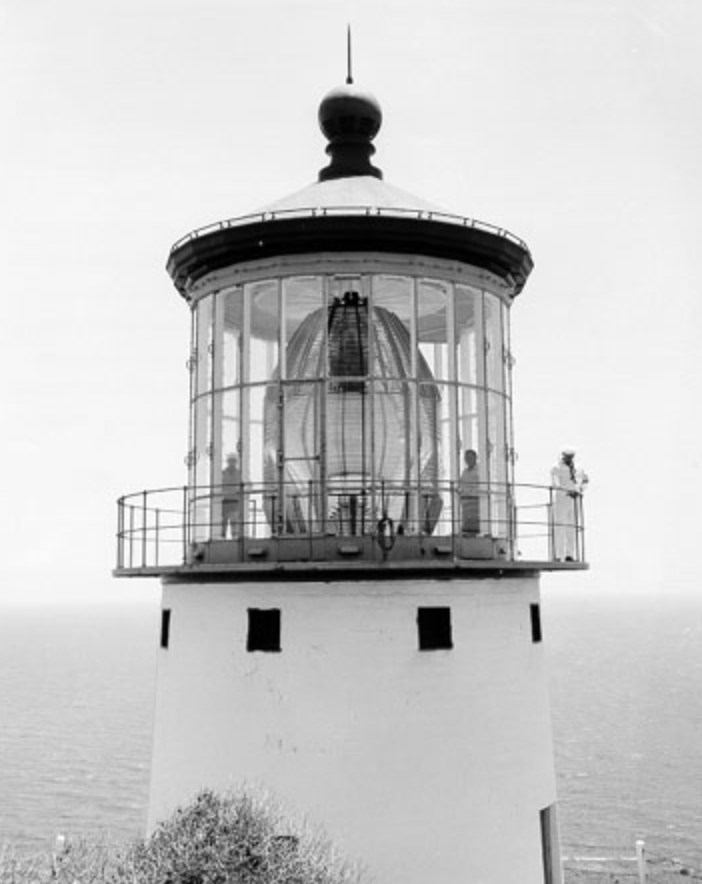
\includegraphics[width=0.2\textwidth]{figures/lighthouse.png}
		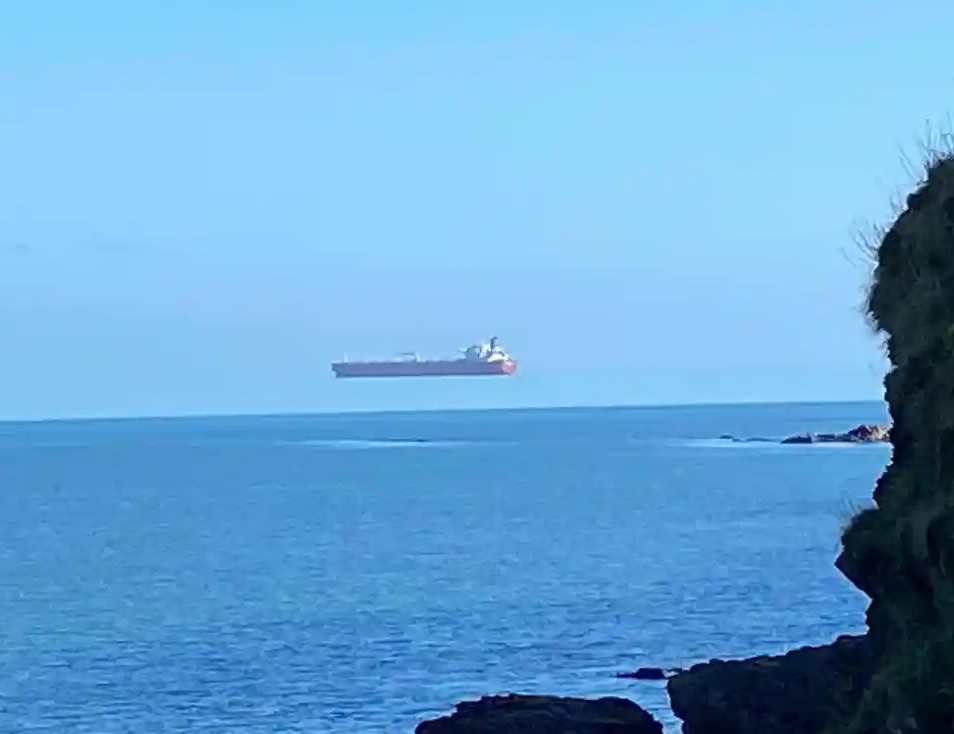
\includegraphics[width=0.327\textwidth]{figures/superior_mirage.png}
		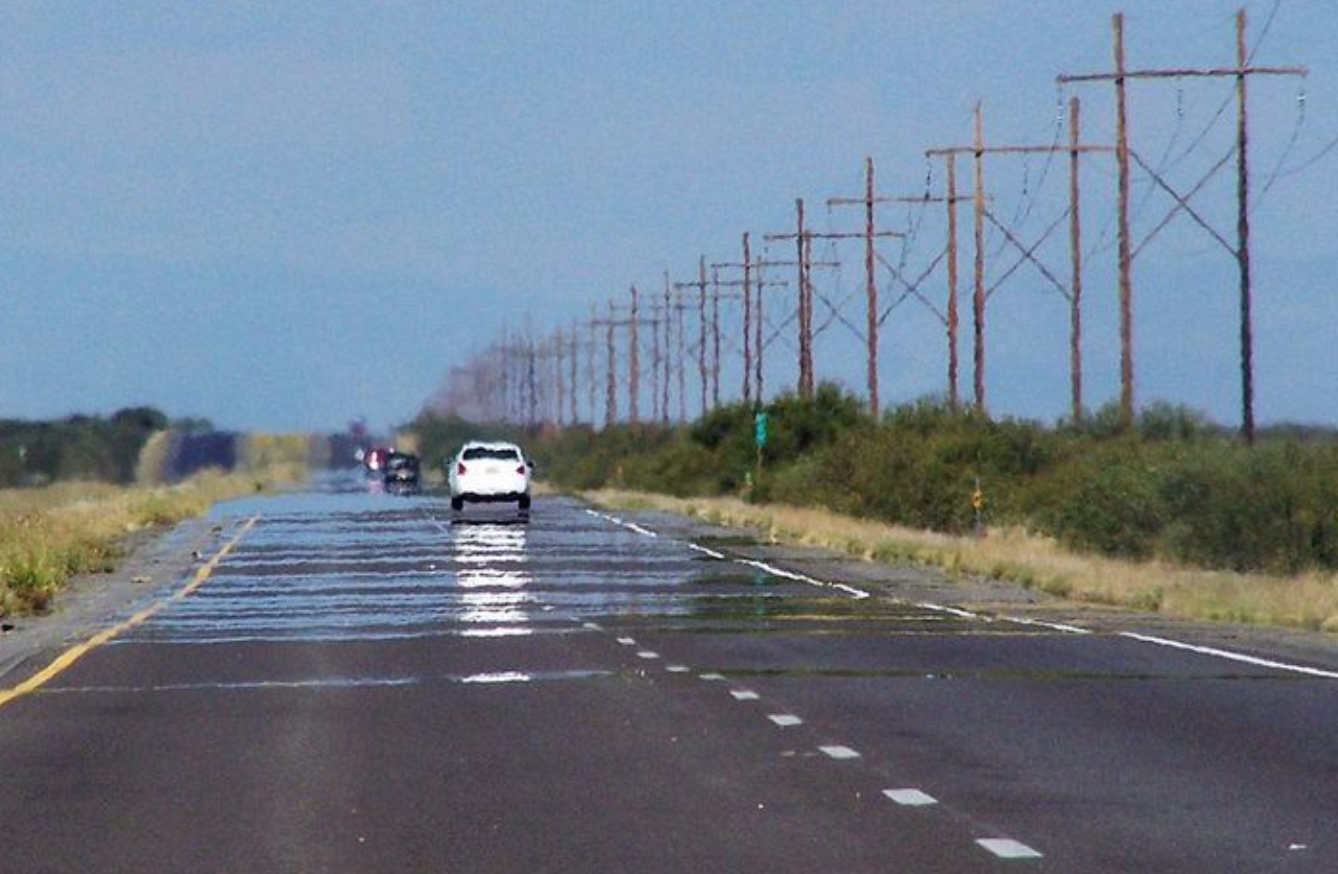
\includegraphics[width=0.385\textwidth]{figures/mirage.png}
		\captionsetup{width=0.93\textwidth}
		\caption{\emph{Left}: A lighthouse with a large high NA lens to collimate light from a lamp at its centre (source: wikipedia). 
		\emph{Middle}: A mirage at sea (photo credit: David Morris).
		\emph{Right}: A mirage on a street (photo credit: Joe Orman).}
		\label{fig:lighthouse_mirage}
	\end{figure}
	
	
	%----------------------------------------------------------------------
    \subsection{Rainbows}
    %----------------------------------------------------------------------
    Explain how rainbows form. What about double rainbows? Draw a sketch.
	
\end{document}
